\documentclass[12pt]{article}
%paquetes del idioma y codificacion
\usepackage[spanish]{babel}
\usepackage[utf8]{inputenc}
\usepackage[T1]{fontenc}
\usepackage{bookman}
%el indice
\usepackage{makeidx}
%paquetes matematicos
\usepackage{amsmath, amsfonts, amssymb}
%dimensiones
\usepackage[left=2.5cm, right=2.5cm, top=2.5cm]{geometry}
%para escribir codigo
\usepackage{listings}
% para contraer referencias
\usepackage{cite}
%para las imagenes y mas...
\usepackage{graphicx}
\usepackage{subfig}
\graphicspath{ {imagenes/} }
\usepackage{float}

\title{Entrega Final de Programas}
\author{Aburto Pérez Luis Mario}
\begin{document}
\maketitle
\newpage
\tableofcontents
\newpage

\section{WEB/EBAY}
\subsection{Descripción del Problema}

Se desea realizar un programa el cual funcione como un buscador de texto, en este caso buscara sub-cadenas dentro de otras. Las cadenas que buscara serán web y ebay. Las cadenas que sean validadas por el autómata las guardara en un archivo además de indicar cuál es su posición con fila y carácter de la fila.

\subsection{Código fuente}
Este programa fue elaborado en el lenguaje Python, su código fuente se muestra a continuación:

Archivo: webay.py
\lstset{language=Python, breaklines=true, basicstyle=\footnotesize}
\begin{lstlisting}[frame=single]

from tkinter import *
from random import *
from grafico import *

def validacion(num):
	if(num>=97 and num<=122):
		return 1
	else:
		return 0

def automata(cadena):
	f=open("estados.txt","a")
	estado=0
	control=0
	if(cadena==''):
		return 0
	else:
		for c in cadena:
			if(estado==0):
				f.write("Estado "+str(estado)+" "+ c+" ")
				if(c=='w'):
					estado=1
				elif(c=='e'):
					estado=4
				else:
					estado=0
			elif(estado==1):
				f.write("Estado "+str(estado)+" "+ c+" ")
				if(c=='e'):
					estado=2
				elif(c=='w'):
					estado=1
				else:
					estado=0
			elif(estado==2):
				f.write("Estado "+str(estado)+" "+ c+" ")
				if(c=='b'):
					estado=3
					control+=1
				elif(c=='e'):
					estado=4
				elif(c=='w'):
					estado=1
				else:
					estado=0
			elif(estado==3):
				f.write("Estado "+str(estado)+" "+ c+" ")
				if(c=='a'):
					estado=6
				elif(c=='e'):
					estado=4
				elif(c=='w'):
					estado=1
				else:
					estado=0
			elif(estado==4):
				f.write("Estado "+str(estado)+" "+ c+" ")
				if(c=='b'):
					estado=5
				elif(c=='e'):
					estado=4
				elif(c=='w'):
					estado=1
			elif(estado==5):
				f.write("Estado "+str(estado)+" "+ c+" ")
				if(c=='a'):
					estado=6
				elif(c=='e'):
					estado=4
				elif(c=='w'):
					estado=1
				else:
					estado=0
			elif(estado==6):
				f.write("Estado "+str(estado)+" "+ c+" ")
				if(c=='y'):
					estado=7
					control+=1
				elif(c=='e'):
					estado=4
				elif(c=='w'):
					estado=1
				else:
					estado=0
			elif(estado==7):
				f.write("Estado "+str(estado)+" "+ c+" ")
				if(c=='w'):
					estado=1
				elif(c=='e'):
					estado=4
	if(control>0):
		return 1
	else:
		return 0

def auto():
	f = open("archivo.txt","r")
	linea=""
	noLinea=1
	control=0
	temporal=''
	linea=f.readline()
	while (linea != ''):
		posTemporal=0
		pos=0
		palabra=linea.lower()
		for c in palabra:
			if(validacion(ord(c))==0):
				control=1
				if(automata(temporal)==1):
					guardarPalabra(pos,linea,noLinea)
				temporal=''
				posTemporal+=1
				pos=posTemporal
			else:
				temporal+=c
				posTemporal+=1
				control=0
		linea=f.readline()
		noLinea+=1
	if(control==0):
		if(automata(temporal)==1):
			guardarPalabra(pos,linea,noLinea)
	f.close()
	f=open("estados.txt","a")
	f.write("\n\n")
	f.close()
	f=open("cadenas.txt","a")
	f.write("\n\n")
	f.close()
	repetir(2)	

def manual():
	control=0
	pos=0
	posTemporal=0
	temporal=''
	cadena=input("Ingresa la cadena ")
	palabra=cadena.lower()
	for c in palabra:
		if(validacion(ord(c))==0):
			control=1
			if(automata(temporal)==1):
				print("Cadena Valida")
				guardarPalabra(pos,cadena,1)
			else:
				print("Cadena Invalida")
			temporal=''
			posTemporal+=1
			pos=posTemporal
		else:
			temporal+=c
			posTemporal+=1
			control=0
	if(control==0):
		if(automata(temporal)==1):
			guardarPalabra(pos,cadena,1)
			print("Cadena Valida")
		else:
			print("Cadena Invalida")
	f=open("estados.txt","a")
	f.write("\n\n")
	f.close()
	f=open("cadenas.txt","a")
	f.write("\n\n")
	f.close()	
	repetir(1)

def guardarPalabra(caracter,cadena,linea):
	f=open("cadenas.txt","a")
	temporal=''
	x=caracter
	while(x<len(cadena) and (validacion(ord(cadena[x].lower()))!=0)):
		temporal+=cadena[x]
		x+=1
	f.write("Fila "+str(linea)+" Caracter "+str(caracter+1)+" "+temporal+" ")
	f.close()

def crearArchivos():
	cadenas=open("cadenas.txt","w")
	cadenas.close()
	estados=open("estados.txt","w")
	estados.close()

def menu():
	crearArchivos()
	eleccion=0
	while (eleccion!=4):
		eleccion=input("Selecciona una opcion\n1.Manual\n2.Automatico\n3.Mostrar Grafico\n4.Salir\n===> ")
		if(eleccion=='1'):
			print("Opcion Manual seleccionada")
			manual()
		elif(eleccion=='2'):
			print("Opcion Automatica seleccionada")
			auto()
		elif(eleccion=='3'):
			print("Visualizar Grafico")
			grafico()
		elif(eleccion=='4'):
			print("Adios")
			return 0
		else:
			print("Opcion Invalida, Intentalo de nuevo")

def repetir(modo):
	rep=''
	if(modo==1):
		while(rep!='1' and rep!='2'):
			rep=input("Deseas Repetir en este modo\n 1. Si \n 2. No\n ==> ")
			if(rep=='1'):
				print("Seleccionaste repetir")
				manual()
			elif(rep=='2'):
				print("Seleccionaste NO repetir")
			else:
				print("Opcion Invalida, Intentalo de nuevo")
	elif(modo==2):
		rep=choice(['1', '2'])
		if(rep=='1'):
			print("Seleccionaste repetir")
			auto()
		elif(rep=='2'):
			print("Seleccionaste NO repetir")

menu()

\end{lstlisting}

\vspace{1em}

Archivo: grafico.py
\lstset{language=Python, breaklines=true, basicstyle=\footnotesize}
\begin{lstlisting}[frame=single]

from tkinter import *
def grafico():
	root = 	Tk()
	root.title('Automata Terminacion "web/ebay" Grafico') # Nombre de la ventana
	canvas=Canvas(root,width=1000,height=700)
	canvas.pack()

	canvas.create_oval(100, 300, 200, 400) #Circulo 0
	canvas.create_arc(180,340,30,360, start=90, extent=180, style='arc') #arco 0-0
	canvas.create_oval(90,355,100,365,fill="red")
	#canvas.create_line(0,350,100,350)#Linea incial
	canvas.create_line(200,340,300,250)#Linea 0-1
	canvas.create_oval(290,250,300,260,fill="red")
	canvas.create_line(200,360,300,450)#Linea 0-4
	canvas.create_oval(290,440,300,450,fill="red")
	canvas.create_arc(150,700,950,0, start=188, extent=149, style='arc') #arco 0-7
	canvas.create_arc(150,600,800,125, start=188, extent=138, style='arc') #arco 0-6
	canvas.create_arc(150,550,600,180, start=190, extent=125, style='arc') #arco 0-5
	canvas.create_arc(150,495,450,265, start=190, extent=92, style='arc') #arco 0-4
	canvas.create_oval(150,400,160,410,fill="red")

	canvas.create_oval(300, 200, 400, 300) #Circulo 1
	canvas.create_line(400,250,500,250)#Linea 1-2
	canvas.create_oval(490,245,500,255,fill="red")
	canvas.create_arc(150,350,340,200, start=45, extent=150, style='arc') #arco 1-0
	canvas.create_oval(145,290,155,300,fill="red")
	canvas.create_arc(370,205,330,160, start=300, extent=300, style='arc') #arco 1-1
	canvas.create_oval(330,195,340,205,fill="red")
	canvas.create_arc(370,205,330,160, start=300, extent=300, style='arc') #arco 1-1

	canvas.create_oval(500, 200, 600, 300) #Circulo 2
	canvas.create_line(600,250,700,250)#Linea 2-3
	canvas.create_oval(690,245,700,255,fill="red")
	canvas.create_arc(525,200,375,240, start=20, extent=140, style='arc') #arco 2-1
	canvas.create_oval(380,205,390,215,fill="red")
	canvas.create_arc(550,150,150,360, start=28, extent=158, style='arc') #arco 2-0
	canvas.create_line(550,300,370,405)#Linea 2-4

	canvas.create_oval(700, 200, 800, 300, width=3) #Circulo 3
	canvas.create_arc(720,70,150,380, start=5, extent=180, style='arc') #arco 3-0
	canvas.create_arc(725,190,380,240, start=10, extent=150, style='arc') #arco 3-1
	canvas.create_line(750,300,370,405)#Linea 3-4
	canvas.create_oval(370,405,380,395,fill="red")

	canvas.create_oval(300, 400, 400, 500) #Circulo 4
	canvas.create_line(400,450,500,450)#Linea 4-5
	canvas.create_oval(490,445,500,455,fill="red")
	canvas.create_arc(290,460,310,480, start=95, extent=255, style='arc') #arco 4-4
	canvas.create_oval(300,480,310,470,fill="red")
	canvas.create_arc(370,450,520,500, start=210, extent=125, style='arc') #arco 4-5
	canvas.create_arc(370,440,720,550, start=180, extent=185, style='arc') #arco 4-6
	canvas.create_arc(370,400,905,600, start=180, extent=173, style='arc') #arco 4-7
	canvas.create_oval(365,495,375,505,fill="red")
	canvas.create_oval(380,485,390,495,fill="red")
	canvas.create_line(350,400,350,300)#Linea 4-1
	canvas.create_oval(345,300,355,310,fill="red")

	canvas.create_oval(500, 400, 600, 500) #Circulo 5
	canvas.create_line(600,450,700,450)#Linea 5-6
	canvas.create_oval(690,445,700,455,fill="red")
	canvas.create_line(550,400,355,305)#Linea 5-1

	canvas.create_oval(700, 400, 800, 500) #Circulo 6
	canvas.create_line(800,450,900,450)#Linea 6-7
	canvas.create_oval(890,445,900,455,fill="red")
	canvas.create_line(750,400,355,305)#Linea 6-1
	canvas.create_line(750,300,770,408)#Linea 3-6
	canvas.create_oval(765,408,775,398,fill="red")

	canvas.create_oval(900,400,1000,500, width=3)#Circulo 7
	canvas.create_line(950,400,355,305)#Linea 7-1

	#Estados
	letra=Label(root,text="Q0",font=("Helvetica",15))
	letra.place(x=125,y=330)
	letra=Label(root,text="Q1",font=("Helvetica",15))
	letra.place(x=330,y=225)
	letra=Label(root,text="Q2",font=("Helvetica",15))
	letra.place(x=530,y=225)
	letra=Label(root,text="Q3",font=("Helvetica",15))
	letra.place(x=730,y=225)
	letra=Label(root,text="Q4",font=("Helvetica",15))
	letra.place(x=330,y=425)
	letra=Label(root,text="Q5",font=("Helvetica",15))
	letra.place(x=530,y=425)
	letra=Label(root,text="Q6",font=("Helvetica",15))
	letra.place(x=730,y=425)
	letra=Label(root,text="Q7",font=("Helvetica",15))
	letra.place(x=930,y=425)
	#Letras e
	letra=Label(root,text="e")
	letra.place(x=250,y=400)
	letra=Label(root,text="e")
	letra.place(x=390,y=375)
	letra=Label(root,text="e")
	letra.place(x=690,y=295)
	letra=Label(root,text="e")
	letra.place(x=280,y=450)
	letra=Label(root,text="e")
	letra.place(x=430,y=490)
	letra=Label(root,text="e")
	letra.place(x=550,y=540)
	letra=Label(root,text="e")
	letra.place(x=690,y=585)
	letra=Label(root,text="e")
	letra.place(x=450,y=230)
	#Letras b
	letra=Label(root,text="b")
	letra.place(x=650,y=230)
	letra=Label(root,text="b")
	letra.place(x=450,y=430)
	#Letras a
	letra=Label(root,text="a")
	letra.place(x=650,y=430)
	letra=Label(root,text="a")
	letra.place(x=750,y=330)
	#Letras y
	letra=Label(root,text="y")
	letra.place(x=850,y=430)
	#Letras compuestas
	letra=Label(root,text="E-e-w")
	letra.place(x=20,y=330)
	letra=Label(root,text="E-e-w")
	letra.place(x=220,y=180)
	letra=Label(root,text="E-b-e-w")
	letra.place(x=270,y=150)
	letra=Label(root,text="E-a-e-w")
	letra.place(x=430,y=80)
	letra=Label(root,text="E-b-e-w")
	letra.place(x=220,y=475)
	letra=Label(root,text="E-a-e-w")
	letra.place(x=320,y=530)
	letra=Label(root,text="E-y-e-w")
	letra.place(x=340,y=570)
	letra=Label(root,text="E-e-w")
	letra.place(x=450,y=650)
	# Letras w
	letra=Label(root,text="w")
	letra.place(x=650,y=180)
	letra=Label(root,text="w")
	letra.place(x=340,y=160)
	letra=Label(root,text="w")
	letra.place(x=450,y=200)
	letra=Label(root,text="w")
	letra.place(x=420,y=330)
	letra=Label(root,text="w")
	letra.place(x=600,y=360)
	letra=Label(root,text="w")
	letra.place(x=850,y=380)
	letra=Label(root,text="w")
	letra.place(x=340,y=350)
	letra=Label(root,text="w")
	letra.pack()
	letra.place(x=250,y=300)
	root.mainloop()

\end{lstlisting}

\newpage
\subsection{Pruebas}
La pruebas que se realizaron sobre este programa fueron 3 una para modo manual, una en modo automàtico y para mostrar su grafico se muestran a continuaciòn: \\

\begin{figure}[H]
\begin{center}
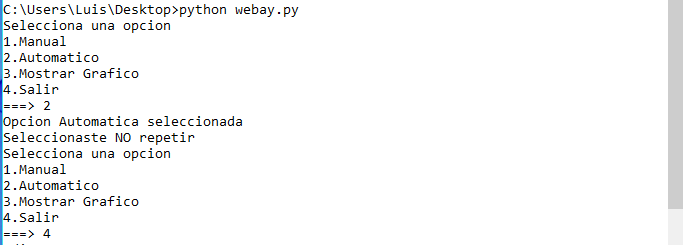
\includegraphics[width=\textwidth, height=8cm]{auto_webay}
\label{fig:auto_webay}
\caption{Modo Automàtico}
\end{center}
\end{figure}

\begin{figure}[H]
\begin{center}
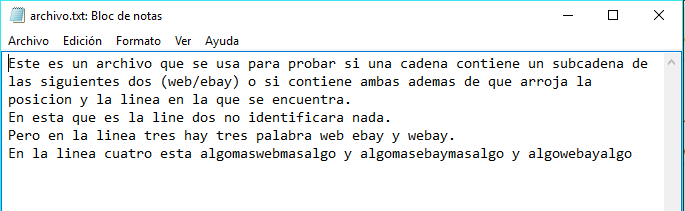
\includegraphics[width=\textwidth, height=8cm]{auto_webay_archivo}
\label{auto_webay_archivo}
\caption{Para el modo automàtico lee un archivo en este caso archivo.txt}
\end{center}
\end{figure}


\begin{figure}[H]
\begin{center}
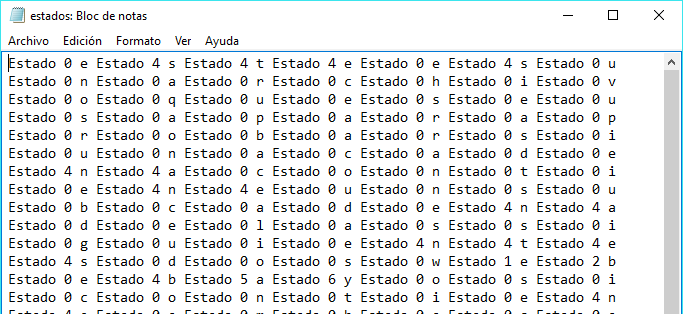
\includegraphics[width=\textwidth, height=8cm]{auto_webay_estado}
\label{ }
\caption{Estados evaluados por el autómata}
\end{center}
\end{figure}


\begin{figure}[H]
\begin{center}
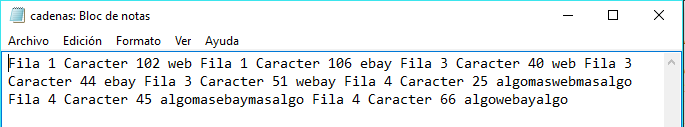
\includegraphics[width=\textwidth, height=8cm]{auto_webay_cadenas}
\label{ }
\caption{Cadenas validas guardadas en el archivo cadenas.txt}
\end{center}
\end{figure}

\begin{figure}[H]
\begin{center}
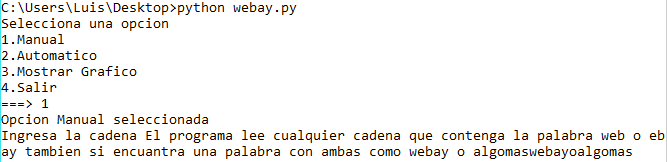
\includegraphics[width=\textwidth, height=8cm]{manual_webay}
\label{fig:auto_webay}
\caption{Modo Manual}
\end{center}
\end{figure}


\begin{figure}[H]
\begin{center}
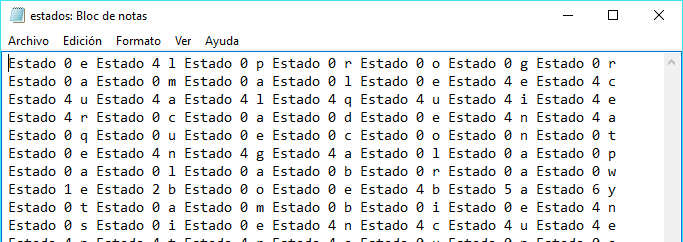
\includegraphics[width=\textwidth, height=8cm]{manual_webay_estados}
\label{ }
\caption{Estados evaluados por el autómata}
\end{center}
\end{figure}


\begin{figure}[H]
\begin{center}
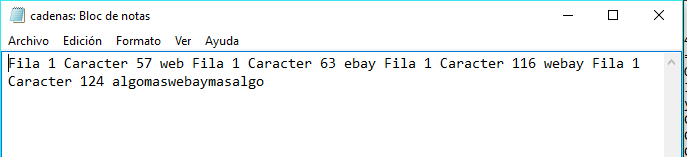
\includegraphics[width=\textwidth, height=8cm]{manual_webay_cadenas}
\label{ }
\caption{Cadenas validas guardadas en el archivo cadenas.txt}
\end{center}
\end{figure}


\begin{figure}[H]
\begin{center}
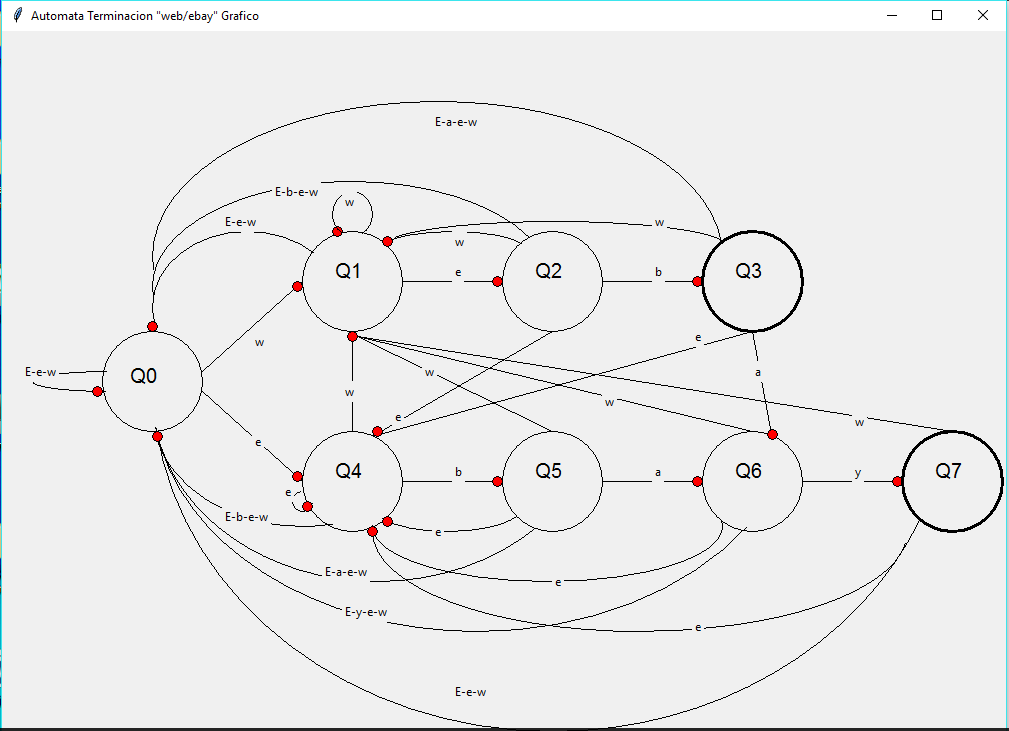
\includegraphics[width=\textwidth, height=11cm]{webay_grafico}
\label{ }
\caption{Gráfico del autòmata}
\end{center}
\end{figure}


\newpage
\section{Planetas}
\subsection{Descripción del Problema}

Se desea realizar un programa el cual de acuerdo a un número n de habitantes genere las combinaciones que son posibles para tres especies dentro del planeta, una vez generadas las combinaciones evaluara la combinación y realizara un proceso para verificar cuales combinaciones fallan y cuáles no, la combinación falla cuando una especie es dominante, es decir, las otras dos especies tiene cero habitantes. El proceso que se aplicara será matar a uno dos especies para añadir dos a la otra especie. El programa solo realizara proceso con combinaciones que no fallen desde el inicio y dará todos los caminos posibles para cada combinación.

\subsection{Código fuente}
Este programa fue elaborado en el lenguaje Python, su código fuente se muestra a continuación:

Archivo: planetas.py
\lstset{language=Python, breaklines=true, basicstyle=\footnotesize}
\begin{lstlisting}[frame=single]

from random import *

def eliminarFinales(listas):
	x=0
	for lista in listas:
		if(lista[0]==0 and lista[1]==0):
			del(listas[x])
		elif(lista[0]==0 and lista[2]==0):
			del(listas[x])
		elif(lista[2]==0 and lista[1]==0):
			del(listas[x])
		x+=1

def generarCombinaciones(listas,n):
	for x in range(0,n+1):
		for y in range(0,n+1):
			for z in range(0,n+1):
				if((x+y+z)==n):
					listas.append([x,y,z])
	eliminarFinales(listas)

def falla(lista):
	if(lista[0]==0 and lista[1]==0):
		return 1
	elif(lista[0]==0 and lista[2]==0):
		return 1
	elif(lista[2]==0 and lista[1]==0):
		return 1
	else:
		return 0

def enRuta(lista,ruta):
	if(ruta==[]):
		return 0
	for casilla in ruta:
		if(casilla==lista):
			return 1
	return 0

def proceso(especie,lista,ruta):
	nueva=lista.copy()
	if(enRuta(nueva,ruta)==1):
		f=open("NoTerminan.txt","a")
		ruta.append(especie)
		ruta.append(lista.copy())
		del(ruta[0])
		f.writelines(str(ruta[0])+" No Termina "+str(ruta)+"\n")
		f.close()
	elif(falla(nueva)==1):
		f=open("Terminan.txt","a")
		ruta.append(especie)
		ruta.append(lista.copy())
		del(ruta[0])
		f.writelines(str(ruta[0])+" TERMINA "+str(ruta)+"\n")
		f.close()
	else:
		ruta.append(especie)
		ruta.append(nueva.copy())
		if(nueva[0]==0):
			nueva[0]+=2
			nueva[1]-=1
			nueva[2]-=1
			proceso("A",nueva.copy(),ruta.copy())
		elif(nueva[1]==0):
			nueva[1]+=2
			nueva[0]-=1
			nueva[2]-=1
			proceso("B",nueva.copy(),ruta.copy())
		elif(nueva[2]==0):
			nueva[2]+=2
			nueva[0]-=1
			nueva[1]-=1
			proceso("C",nueva.copy(),ruta.copy())
		else:
			nueva1=nueva.copy()
			nueva2=nueva.copy()
			nueva3=nueva.copy()
			nueva1[0]+=2
			nueva1[1]-=1
			nueva1[2]-=1
			proceso("A",nueva1.copy(),ruta.copy())
			nueva2[1]+=2
			nueva2[0]-=1
			nueva2[2]-=1
			proceso("B",nueva2.copy(),ruta.copy())
			nueva3[2]+=2
			nueva3[0]-=1
			nueva3[1]-=1
			proceso("C",nueva3.copy(),ruta.copy())

def crearArchivo():
	f=open("Terminan.txt","w")
	f.close()
	f=open("NoTerminan.txt","w")
	f.close()

def manual():
	listas=[]
	habitantes=0
	habitantes=int(input("Ingresa el numero de habitantes en el planeta (2-15) ==>  "))
	while(habitantes>15 or habitantes<2):
		print("Opcion Invalida")
		habitantes=int(input("Ingresa el numero de habitantes en el planeta (2-15) ==>  "))
	f=open("Terminan.txt","a")
	g=open("NoTerminan.txt","a")
	generarCombinaciones(listas,habitantes)
	for lista in listas:
		ruta=[]
		proceso("A",lista,ruta)
	f.write("Termina Ejecucion\n")
	g.write("Termina Ejecucion\n")
	f.close()
	g.close()
	repetir(1)

def auto():
	listas=[]
	habitantes=randint(2,15)
	f=open("Terminan.txt","a")
	g=open("NoTerminan.txt","a")
	print("El numero seleccionado es " +str(habitantes))
	generarCombinaciones(listas,habitantes)
	f.write("Termina Ejecucion\n")
	g.write("Termina Ejecucion\n")
	for lista in listas:
		ruta=[]
		proceso("A",lista,ruta)
	f.close()
	g.close()
	repetir(2)

def menu():
	eleccion=0
	crearArchivo()
	while (eleccion!=4):
		eleccion=input("Selecciona una opcion\n1.Manual\n2.Automatico\n3.Salir\n===> ")
		if(eleccion=='1'):
			print("Opcion Manual seleccionada")
			manual()
		elif(eleccion=='2'):
			print("Opcion Automatica seleccionada")
			auto()
		elif(eleccion=='3'):
			print("Adios")
			return 0
		else:
			print("Opcion Invalida, Intentalo de nuevo")

def repetir(modo):
	rep=''
	if(modo==1):
		while(rep!='1' and rep!='2'):
			rep=input("Deseas Repetir en este modo\n 1. Si \n 2. No\n ==> ")
			if(rep=='1'):
				print("Seleccionaste repetir")
				manual()
			elif(rep=='2'):
				print("Seleccionaste NO repetir")
			else:
				print("Opcion Invalida, Intentalo de nuevo")
	elif(modo==2):
		rep=choice(['1', '2'])
		if(rep=='1'):
			print("Seleccionaste repetir")
			auto()
		elif(rep=='2'):
			print("Seleccionaste NO repetir")
menu()

\end{lstlisting}

\subsection{Pruebas}
Para este programa se realizaron dos pruebas, en su modo automático donde el número de habitantes es generado por un random y otro en el modo manual que es ingresado por el usuario. También se mostrara todos los caminos posibles que son tomados por la combinaciones generadas.  \\

\begin{figure}[H]
\begin{center}
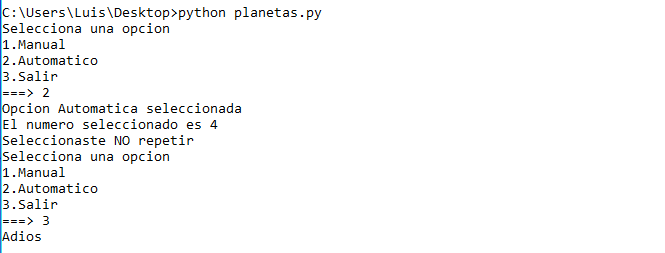
\includegraphics[width=\textwidth, height=8cm]{auto_planetas}
\label{ }
\caption{Modo Automático}
\end{center}
\end{figure}

\begin{figure}[H]
\begin{center}
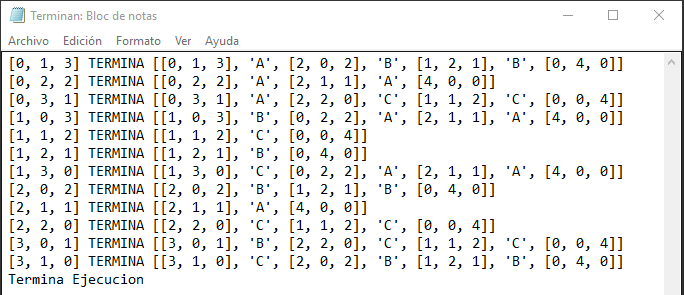
\includegraphics[width=\textwidth, height=8cm]{auto_planetas_fallan}
\label{ }
\caption{Combinaciones que fallan con su proceso.}
\end{center}
\end{figure}

\begin{figure}[H]
\begin{center}
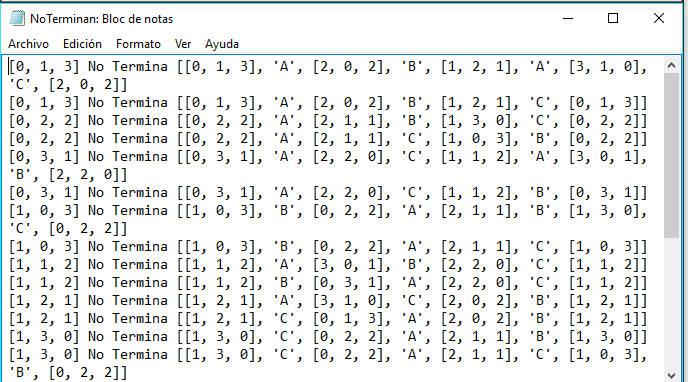
\includegraphics[width=\textwidth, height=8cm]{auto_planetas_nofallan}
\label{ }
\caption{Combinaciones que no fallan con su proceso.}
\end{center}
\end{figure}

\begin{figure}[H]
\begin{center}
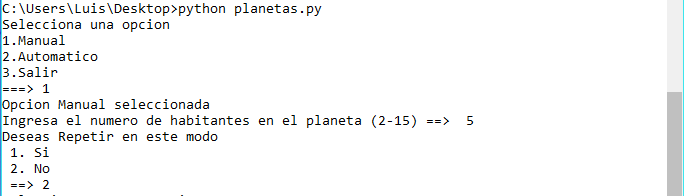
\includegraphics[width=\textwidth, height=8cm]{manual_planetas}
\label{ }
\caption{Modo Manual}
\end{center}
\end{figure}

\begin{figure}[H]
\begin{center}
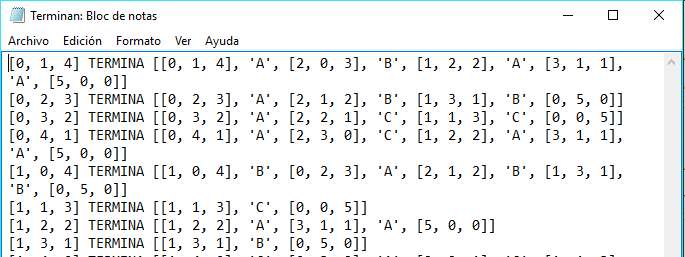
\includegraphics[width=\textwidth, height=8cm]{manual_planetas_fallan}
\label{ }
\caption{Combinaciones que fallan con su proceso.}
\end{center}
\end{figure}

\begin{figure}[H]
\begin{center}
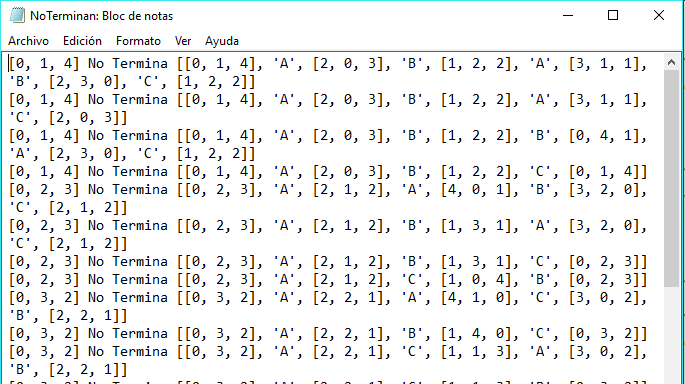
\includegraphics[width=\textwidth, height=8cm]{manual_planetas_nofallan}
\label{ }
\caption{Combinaciones que no fallan con su proceso.}
\end{center}
\end{figure}

\newpage
\section{Palindromo}
\subsection{Descripción del Problema}

Se desea hacer un programa que genere un palíndromo (cadena que es igual al leerla de izquierda a derecha como leerla de derecha a izquierda)  binario, es decir, de 0’s y 1’s. La cadena que se generara será dependiendo de un numero el cual es la longitud de la cadena además de indicar el número de veces que entrara en el proceso la cadena. La cadena será generada por reglas de producción que serán tomadas de forma aleatoria.

\subsection{Código fuente}
Este programa fue elaborado en el lenguaje Python, su código fuente se muestra a continuación:

Archivo: palindromo.py
\lstset{language=Python, breaklines=true, basicstyle=\footnotesize}
\begin{lstlisting}[frame=single]

from random import *
def generarCadena(n):
	f=open("proceso.txt","a")
	cadena=""
	if(n%2==0):
		rep=0
		while(rep<(n/2)):
			numero=randint(1,2)
			if(numero==1):
				cadena+="0"
				cadenaDos=invertir(cadena)
				#print(" 0P0 | "+cadena+"P"+cadenaDos)
				f.write(" 0P0 | "+cadena+"P"+cadenaDos+"\n")
			if(numero==2):
				cadena+="1"
				cadenaDos=invertir(cadena)
				#print(" 1P1 | "+cadena+"P"+cadenaDos)
				f.write(" 1P1 | "+cadena+"P"+cadenaDos+"\n")
			rep+=1
		cadenaDos=invertir(cadena)
		#print("  e  | "+cadena+"e"+cadenaDos)
		f.write("  e  | "+cadena+"e"+cadenaDos+"\n")
		cadena=cadena+cadenaDos
	else:
		rep=0
		while(rep<(n/2)-0.5):
			numero=randint(1,2)
			if(numero==1):
				cadena+="0"
				cadenaDos=invertir(cadena)
				#print(" 0P0 | "+cadena+"P"+cadenaDos)
				f.write(" 0P0 | "+cadena+"P"+cadenaDos+"\n")
			if(numero==2):
				cadena+="1"
				cadenaDos=invertir(cadena)
				#print(" 1P1 | "+cadena+"P"+cadenaDos)
				f.write(" 1P1 | "+cadena+"P"+cadenaDos+"\n")
			rep+=1
		cadenaDos=invertir(cadena)
		numero=randint(1,2)
		if(numero==1):
			cadena+="0"
			cadena=cadena+cadenaDos
			#print("  0  | "+cadena)
			f.write("  0  | "+cadena+"\n")
		elif(numero==2):
			cadena+="1"
			cadena=cadena+cadenaDos
			#print("  1  | "+cadena)
			f.write("  1  | "+cadena+"\n")
	print("El palindromo binario generado es "+cadena)
	f.write("El palindromo binario generado es "+cadena+"\n\n")
	f.close()

def invertir(cadena):
        return cadena[::-1]

def crearArchivo():
	f=open("proceso.txt","w")
	f.close()

def menu():
	crearArchivo()
	eleccion=0
	while (eleccion!=4):
		eleccion=input("Selecciona una opcion\n1.Manual\n2.Automatico\n3.Salir\n===> ")
		if(eleccion=='1'):
			print("Opcion Manual seleccionada")
			manual()
		elif(eleccion=='2'):
			print("Opcion Automatica seleccionada")
			auto()
		elif(eleccion=='3'):
			print("Adios")
			return 0
		else:
			print("Opcion Invalida, Intentalo de nuevo")

def manual():
	numero=int(input("Ingresa el numero "))
	generarCadena(numero)
	repetir(1)

def auto():
	numero=randint(0,1000)
	print("El numero seleccionado es "+str(numero))
	generarCadena(numero)
	repetir(2)

def repetir(modo):
	rep=''
	if(modo==1):
		while(rep!='1' and rep!='2'):
			rep=input("Deseas Repetir en este modo\n 1. Si \n 2. No\n ==> ")
			if(rep=='1'):
				print("Seleccionaste repetir")
				manual()
			elif(rep=='2'):
				print("Seleccionaste NO repetir")
			else:
				print("Opcion Invalida, Intentalo de nuevo")
	elif(modo==2):
		rep=choice(['1', '2'])
		if(rep=='1'):
			print("Seleccionaste repetir")
			auto()
		elif(rep=='2'):
			print("Seleccionaste NO repetir")

menu()

\end{lstlisting}

\subsection{Pruebas}

Para este programa se realizaron dos pruebas, en su modo automático que generara la longitud de la cadena a través de un random y otro en el modo manual donde el nùmero es ingresado por el usuario. Además de mostrar el proceso por el cual es generado el palíndromo.

\begin{figure}[H]
\begin{center}
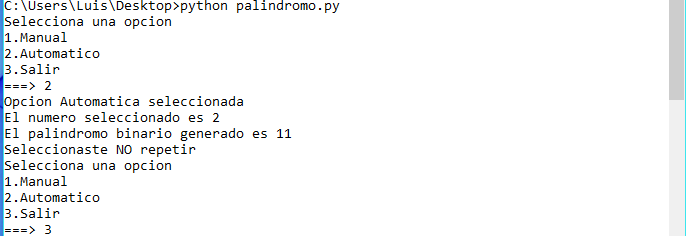
\includegraphics[width=\textwidth, height=8cm]{auto_palindromo}
\label{ }
\caption{Modo Automático}
\end{center}
\end{figure}

\begin{figure}[H]
\begin{center}
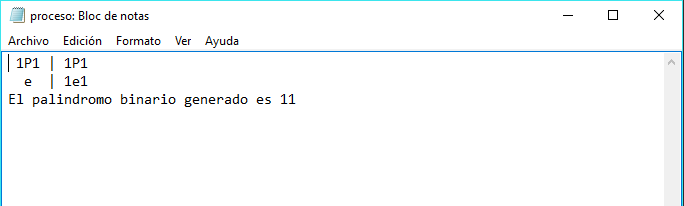
\includegraphics[width=\textwidth, height=8cm]{auto_palindromo_proceso}
\label{ }
\caption{Proceso por el cual es formado el palíndromo.}
\end{center}
\end{figure}

\begin{figure}[H]
\begin{center}
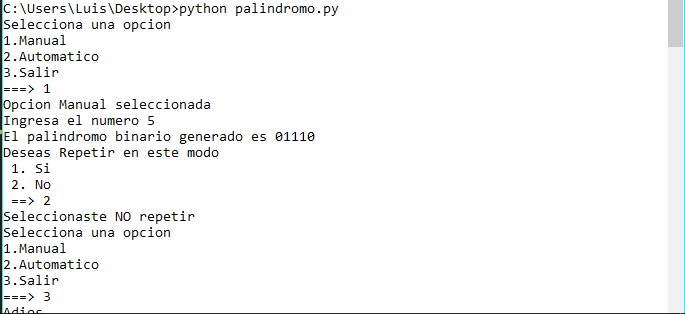
\includegraphics[width=\textwidth, height=8cm]{manual_palindromo}
\label{ }
\caption{Modo Manual}
\end{center}
\end{figure}

\begin{figure}[H]
\begin{center}
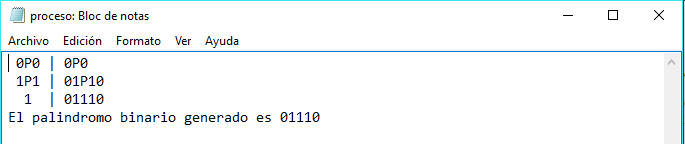
\includegraphics[width=\textwidth, height=8cm]{manual_palindromo_proceso}
\label{ }
\caption{Proceso por el cual es formado el palíndromo.}
\end{center}
\end{figure}

\newpage
\section{Parentesis}
\subsection{Descripción del Problema}

Se desea realizar un programa el cual evalué si una cadena esta balanceada en cuanto al número de paréntesis que abren y cierran. La evaluación se hará dependiendo de las reglas de producción que se tienen, dependiendo del carácter que se lea será la regla que se utilizara para la evaluación que será ir sustituyendo el carácter que llega por la regla de producción y al final encontrar si la cadena es válida o no, es decir, si esta balanceada en los paréntesis.

\subsection{Código fuente}
Este programa fue elaborado en el lenguaje Python, su código fuente se muestra a continuación:
Archivo: parentesis.py
\lstset{language=Python, breaklines=true, basicstyle=\footnotesize}
\begin{lstlisting}[frame=single]

from random import*

def imprimir(lista,c,regla):
	f=open("proceso.txt","a")
	cad=""
	for x in lista:
		cad+=x
	while(len(c)!=20):
		c+=" "
	if(regla==0):
		f.write("Inicio | "+c + " | "+cad+"\n")
	elif(regla==1):
		f.write("B->(RB | "+c + " | "+cad+"\n")
	elif(regla==2):
		f.write("B-> e  | "+c + " | "+cad+"\n")
	elif(regla==3):
		f.write("R->(RR | "+c + " | "+cad+"\n")
	elif(regla==4):
		f.write("R-> )  | "+c + " | "+cad+"\n")
	f.close()

def acomodarCadena(cadena):
	cadenaAux=""
	if(cadena==""):
		return "Resultado"
	for x in range(1,len(cadena)):
		cadenaAux+=cadena[x]
	return cadenaAux

def automata(cadena):
	cadenaAux=cadena
	regla=0
	pasos=['B']
	imprimir(pasos,cadena,regla)
	for c in cadena:
		cadenaAux=acomodarCadena(cadenaAux)
		x=0
		while(pasos[x]=='(' or pasos[x]==')'):
			x+=1
		estado=pasos[x]
		if(estado=='B'):
			if(c=='('):
				pasos.insert(x,'(')
				pasos.remove('B')
				pasos.append('R')
				pasos.append('B')
				regla=1
			elif(c==')'):
				return 0						
		elif(estado=='R'):
			if(c=='('):
				pasos.insert(x-1,'(')
				pasos.insert(x+1,'R')
				regla=3
			if(c==')'):
				pasos.insert(x,')')
				pasos.remove('R')
				regla=4
		imprimir(pasos,cadenaAux,regla)
	if(pasos[-2]==')' and pasos[-1]=='B'):
		pasos.remove('B')
		imprimir(pasos,acomodarCadena(cadenaAux),2)
		return 1
	else:
		return 0

def crearArchivo():
	f=open("proceso.txt","w")
	f.close()

def menu():
	crearArchivo()
	eleccion=0
	while (eleccion!=4):
		eleccion=input("Selecciona una opcion\n1.Manual\n2.Automatico\n3.Salir\n===> ")
		if(eleccion=='1'):
			print("Opcion Manual seleccionada")
			manual()
		elif(eleccion=='2'):
			print("Opcion Automatica seleccionada")
			auto()
		elif(eleccion=='3'):
			print("Adios")
			return 0
		else:
			print("Opcion Invalida, Intentalo de nuevo")

def manual():
	f=open("proceso.txt","a")
	cadena=input("Ingresa la cadena ")
	if(automata(cadena)==1):
		print("La cadena "+cadena+" es Valida")
		f.write("La cadena "+cadena+" es Valida\n\n")
	else:
		print("La cadena "+cadena+" NO esta balanceada")
		f.write("La cadena "+cadena+" NO esta balanceada\n\n")
	f.close()
	repetir(1)


def auto():
	cadena=generarCadena()
	f=open("proceso.txt","a")
	if(automata(cadena)==1):
		print("La cadena "+cadena+" es Valida")
		f.write("La cadena "+cadena+" es Valida\n\n")
	else:
		print("La cadena "+cadena+" NO esta balanceada")
		f.write("La cadena "+cadena+" NO esta balanceada\n\n")
	f.close()
	repetir(2)

def generarCadena():
    longitud=randint(1,20)
    cadena=''
    i=0
    while(i<longitud):
	    cadena+=choice(['(', ')'])
	    i += 1
    print("La cadena generado es: "+cadena)
    return cadena

def repetir(modo):
	rep=''
	if(modo==1):
		while(rep!='1' and rep!='2'):
			rep=input("Deseas Repetir en este modo\n 1. Si \n 2. No\n ==> ")
			if(rep=='1'):
				print("Seleccionaste repetir")
				manual()
			elif(rep=='2'):
				print("Seleccionaste NO repetir")
			else:
				print("Opcion Invalida, Intentalo de nuevo")
	elif(modo==2):
		rep=choice(['1', '2'])
		if(rep=='1'):
			print("Seleccionaste repetir")
			auto()
		elif(rep=='2'):
			print("Seleccionaste NO repetir")

menu()

\end{lstlisting}

\subsection{Pruebas}

Para este programa se realizaron dos pruebas, en su modo automático que generara una cadena de paréntesis la cual luego verificara si está o no balanceada y la otra será en modo manual en la cual el usuario ingresara la cadena para validar. \\

\begin{figure}[H]
\begin{center}
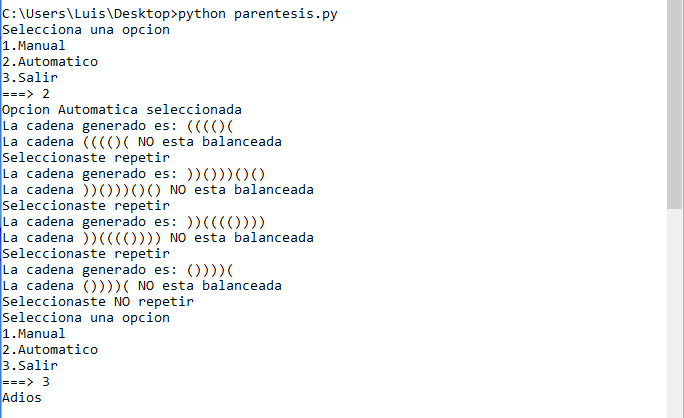
\includegraphics[width=\textwidth, height=8cm]{auto_parentesis}
\label{ }
\caption{Modo Automático}
\end{center}
\end{figure}

\begin{figure}[H]
\begin{center}
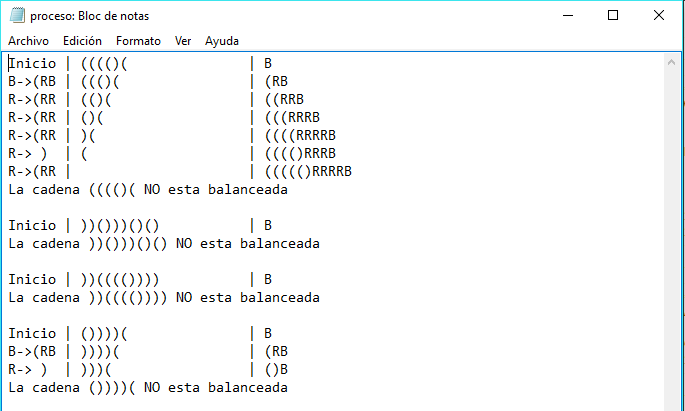
\includegraphics[width=\textwidth, height=8cm]{auto_parentesis_proceso}
\label{ }
\caption{Proceso de evaluación.}
\end{center}
\end{figure}

\begin{figure}[H]
\begin{center}
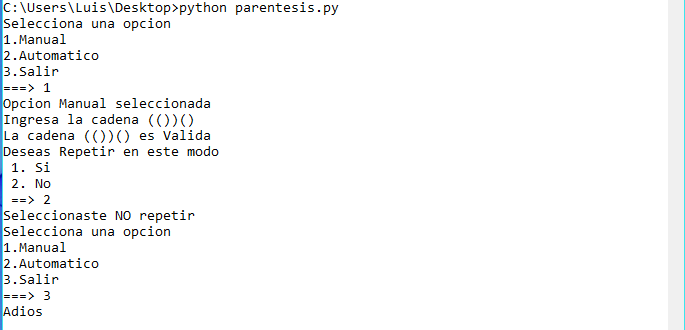
\includegraphics[width=\textwidth, height=8cm]{manual_parentesis}
\label{ }
\caption{Modo Manual}
\end{center}
\end{figure}

\begin{figure}[H]
\begin{center}
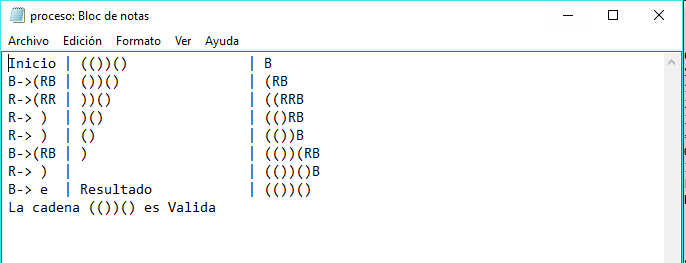
\includegraphics[width=\textwidth, height=8cm]{manual_parentesis_proceso}
\label{ }
\caption{Proceso de evaluación.}
\end{center}
\end{figure}

\newpage
\section{Pila}
\subsection{Descripción del Problema}

Se desea realizar un programa que emplee el autómata de pila. Para este programa se realizara una clase llamada Pila que tendrá las funciones típicas de este tipo de dato abstracto como el visto en el curso de Estructura de Datos en el semestre anterior. La pila evaluara una secuencia de ceros y unos manejando estados de la pila, caracteres que entran y salen a la pila, en este caso una ‘X’. Cada vez que vea un cero se realizara un push() y cada uno un pop() al final se evaluara si la pila esta vacía. Lo que indicara que la cadena es válida.

\subsection{Código fuente}
Este programa fue elaborado en el lenguaje Python, su código fuente se muestra a continuación:
Archivo: pila.py
\lstset{language=Python, breaklines=true, basicstyle=\footnotesize}
\begin{lstlisting}[frame=single]

#Pila
class Pila:
	lista=[]
	tope=0
	estado=""

	def inicializarPila(self):
		self.lista.append('Zo')
		self.lista.append(None)
		self.tope=1
		self.estado="q"

	def push(self):
		self.lista[self.tope]='X'
		self.lista.append(None)
		self.tope+=1

	def pop(self):
		del(self.lista[self.tope])
		self.tope-=1
		self.lista[self.tope]=None

	def mostrar(self):
		cad=""
		x=len(self.lista)-2
		while(x>=0):
			cad+=str(self.lista[x])
			x-=1
		return cad

	def esVacia(self):
		if(self.tope==1):
			return 1
		else:
			return 0

\end{lstlisting}

Archivo: aPila.py
\lstset{language=Python, breaklines=true, basicstyle=\footnotesize}
\begin{lstlisting}[frame=single]

from time import *
from Pila import *
from random import *
from tkinter import *

def automata(pila,cadena):
	f=open("historial.txt","a")
	root = 	Tk()
	root.title('Grafico') # Nombre de la ventana
	canvas=Canvas(root,width=510,height=500)
	canvas.pack()
	canvas.create_line(175,150,175,50)
	canvas.create_line(175,300,175,400)
	estado=Label(root,text="     ",bg="black",font=("Helvetica",100))
	estado.place(x = 100, y = 150)
	pila.estado="q"
	cadenaAux=cadena
	f.write("("+pila.estado+","+cadena+","+pila.mostrar()+")|-")
	estado=Label(root,text="                              ",font=("Helvetica",15))
	estado.place(x = 170, y = 35)
	estado=Label(root,text="                              ",font=("Helvetica",15))
	estado.place(x = 170, y = 400)
	estado=Label(root,text=cadenaAux,font=("Helvetica",15))
	estado.place(x = 170, y = 35)
	estado=Label(root,text=pila.mostrar(),font=("Helvetica",15))
	estado.place(x = 170, y = 400)
	estado=Label(root,text=pila.estado+"  ",bg="black",font=("Helvetica",25),fg="white")
	estado.place(x = 175, y = 200)
	root.update()
	sleep(1)
	for x in cadena:
		if(x=='0'):
			pila.estado='q'
			pila.push()
			cadenaAux=eliminarCaracter(cadenaAux)
			f.write("("+pila.estado+","+cadenaAux+","+pila.mostrar()+")|-")
			estado=Label(root,text="                              ",font=("Helvetica",15))
			estado.place(x = 170, y = 35)
			estado=Label(root,text="                              ",font=("Helvetica",15))
			estado.place(x = 170, y = 400)
			estado=Label(root,text=cadenaAux,font=("Helvetica",15))
			estado.place(x = 170, y = 35)
			estado=Label(root,text=pila.mostrar(),font=("Helvetica",15))
			estado.place(x = 170, y = 400)
			estado=Label(root,text=pila.estado+"  ",bg="black",font=("Helvetica",25),fg="white")
			estado.place(x = 175, y = 200)
			root.update()
			sleep(1)
		elif(x=='1'):
			if(pila.tope>1):
				pila.pop()
				pila.estado='p'
				cadenaAux=eliminarCaracter(cadenaAux)
				f.write("("+pila.estado+","+cadenaAux+","+pila.mostrar()+")|-")
				estado=Label(root,text="                              ",font=("Helvetica",15))
				estado.place(x = 170, y = 35)
				estado=Label(root,text="                              ",font=("Helvetica",15))
				estado.place(x = 170, y = 400)
				estado=Label(root,text=cadenaAux,font=("Helvetica",15))
				estado.place(x = 170, y = 35)
				estado=Label(root,text=pila.mostrar(),font=("Helvetica",15))
				estado.place(x = 170, y = 400)
				estado=Label(root,text=pila.estado+"  ",bg="black",font=("Helvetica",25),fg="white")
				estado.place(x = 175, y = 200)
				root.update()
				sleep(1)
			else:
				root.mainloop()
				f.write("\n")
				f.close()
				return 0
	if(pila.esVacia()==1):
		pila.estado='f'
		f.write("("+pila.estado+","+cadenaAux+","+pila.mostrar()+")\n\n")
		estado=Label(root,text="                              ",font=("Helvetica",15))
		estado.place(x = 170, y = 35)
		estado=Label(root,text="                              ",font=("Helvetica",15))
		estado.place(x = 170, y = 400)
		estado=Label(root,text=cadenaAux,font=("Helvetica",15))
		estado.place(x = 170, y = 35)
		estado=Label(root,text=pila.mostrar(),font=("Helvetica",15))
		estado.place(x = 170, y = 400)
		estado=Label(root,text=pila.estado+"  ",bg="black",font=("Helvetica",25),fg="white")
		estado.place(x = 175, y = 200)
		root.update()
		sleep(1)
		root.mainloop()
		f.write("\n")
		f.close()
		return 1

def eliminarCaracter(cadena):
	x=1
	cadenaAux=""
	while(x<len(cadena)):
		cadenaAux+=cadena[x]
		x+=1
	if(cadenaAux==""):
		return "epsilon"
	else:
		return cadenaAux

def manual(pila):
	f=open("cadenas.txt","a")
	cadena=input("Ingresa la cadena ")
	if(automata(pila,cadena)==1):
		print("Cadena Valida")
		f.write(cadena+" Cadena Valida\n\n")
	else:
		print("Cadena Invalida")
		f.write(cadena+" Cadena Invalida\n\n")
	f.close()
	repetir(1,pila)

def auto(pila):
	f=open("cadenas.txt","a")
	cadena=generarCadena()
	if(automata(pila,cadena)==1):
		print("Cadena Valida")
		f.write(cadena+" Cadena Valida\n\n")
	else:
		print("Cadena Invalida")
		f.write(cadena+" Cadena Invalida\n\n")
	f.close()
	repetir(2,pila)

def generarCadena():
    longitud=randint(1,1000)
    numero=''
    i=0
    while(i<longitud):
	    numero+=choice(['0', '1'])
	    i += 1
    print("El numero generado es: "+numero)
    return numero

def repetir(modo,pila):
	rep=''
	if(modo==1):
		while(rep!='1' and rep!='2'):
			rep=input("Deseas Repetir en este modo\n 1. Si \n 2. No\n ==> ")
			if(rep=='1'):
				print("Seleccionaste repetir")
				manual(pila)
			elif(rep=='2'):
				print("Seleccionaste NO repetir")
			else:
				print("Opcion Invalida, Intentalo de nuevo")
	elif(modo==2):
		rep=choice(['1', '2'])
		if(rep=='1'):
			print("Seleccionaste repetir")
			auto(pila)
		elif(rep=='2'):
			print("Seleccionaste NO repetir")

def crearArchivo():
	f=open("historial.txt","w")
	f.close()
	f=open("cadenas.txt","w")
	f.close()

def menu(pila):
	crearArchivo()
	eleccion=0
	while (eleccion!=4):
		eleccion=input("Selecciona una opcion\n1.Manual\n2.Automatico\n3.Salir\n===> ")
		if(eleccion=='1'):
			print("Opcion Manual seleccionada")
			manual(pila)
		elif(eleccion=='2'):
			print("Opcion Automatica seleccionada")
			auto(pila)
		elif(eleccion=='3'):
			print("Adios")
			return 0
		else:
			print("Opcion Invalida, Intentalo de nuevo")

pila=Pila()
pila.inicializarPila()
menu(pila)

\end{lstlisting}

\subsection{Pruebas}

Para este programa se realizaron dos pruebas, en su modo automático que generara una cadena binaria la cual luego verificara si tiene o no el mismo número de 1’s y 0’s y la otra será en modo manual en la cual el usuario ingresara la cadena para validar. Además se mostrara el proceso en modo gráfico.\\

\begin{figure}[H]
\begin{center}
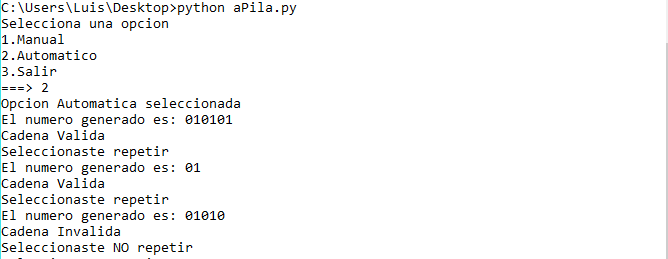
\includegraphics[width=\textwidth, height=8cm]{auto_pila}
\label{ }
\caption{Modo Automático}
\end{center}
\end{figure}

\begin{figure}[H]
\begin{center}
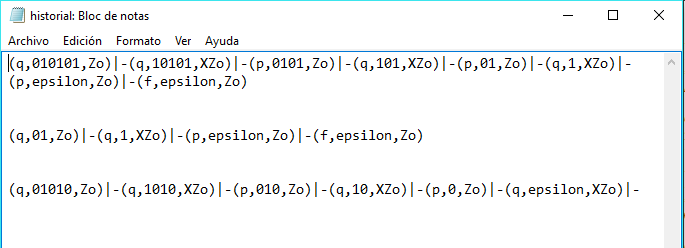
\includegraphics[width=\textwidth, height=8cm]{auto_pila_historial}
\label{ }
\caption{Historial de estados y caracteres por los cuales pasa la pila.}
\end{center}
\end{figure}

\begin{figure}[H]
\begin{center}
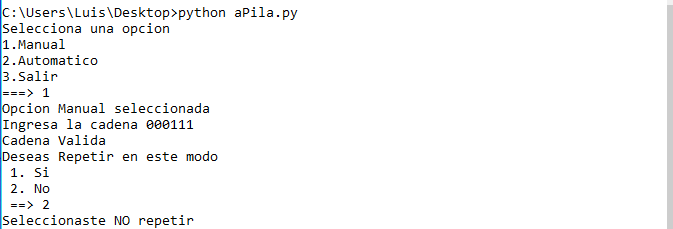
\includegraphics[width=\textwidth, height=8cm]{manual_pila}
\label{ }
\caption{Modo Manual}
\end{center}
\end{figure}

\begin{figure}[H]
\begin{center}
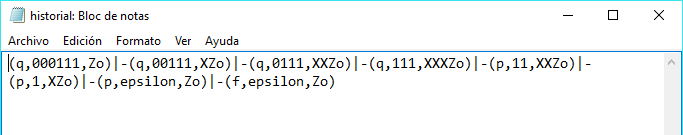
\includegraphics[width=\textwidth, height=8cm]{manual_pila_historial}
\label{ }
\caption{Historial de estados y caracteres por los cuales pasa la pila.}
\end{center}
\end{figure}

\begin{figure}[H]
\begin{center}
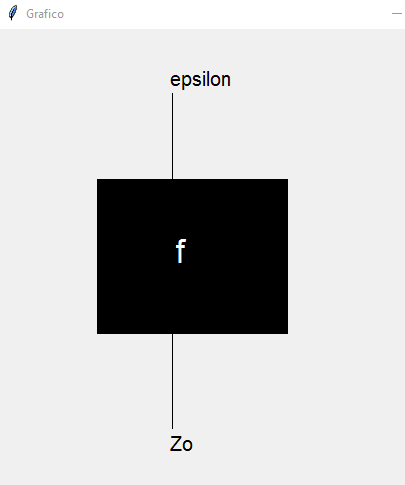
\includegraphics[width=\textwidth, height=15cm]{grafico_pila}
\label{ }
\caption{Grafico Pila.}
\end{center}
\end{figure}

\newpage
\section{Máquina de Turing}
\subsection{Descripción del Problema}

Se desea emplear una máquina de Turing que evalué si una cadena está compuesta de la siguiente forma \[0^{n}1^{n}\]El proceso que seguirá la máquina de Turing es cambiar los ceros por X’s y los unos por Y’s al final evaluara si la cadena cumple con esa regla. La forma en la que se procesara la cadena será a través de estados los cuales cambiaran los caracteres y se moveran a la derecha o izquierda de la cadena para evaluar la cadena de forma correcta.

\subsection{Código fuente}
Este programa fue elaborado en el lenguaje Python, su código fuente se muestra a continuación:

Archivo: turing.py
\lstset{language=Python, breaklines=true, basicstyle=\footnotesize}
\begin{lstlisting}[frame=single]

from random import *

def automata(c):
	c.append('B')
	pos=0
	f=open("proceso.txt","a")
	estado=0
	mov=' '
	while(pos<len(c)):
		f.write("(q"+str(estado)+","+c[pos]+","+mov+")\n")
		f.write(pasarCadena(c.copy(),pos,estado)+"\n")
		if(estado==0):
			if(c[pos]=='0'):
				estado=1
				c[pos]='X'
				pos+=1
				mov='R'
			elif(c[pos]=='Y'):
				estado=3
				c[pos]='Y'
				pos+=1
				mov='R'
			else:
				return 0
		elif(estado==1):
			if(c[pos]=='0'):
				estado=1
				c[pos]='0'
				pos+=1
				mov='R'
			elif(c[pos]=='1'):
				estado=2
				c[pos]='Y'
				pos-=1
				mov='L'
			elif(c[pos]=='Y'):
				estado=1
				c[pos]='Y'
				pos+=1
				mov='R'
			else:
				return 0
		elif(estado==2):
			if(c[pos]=='0'):
				estado=2
				c[pos]='0'
				pos-=1
				mov='L'
			elif(c[pos]=='X'):
				estado=0
				c[pos]='X'
				pos+=1
				mov='R'
			elif(c[pos]=='Y'):
				estado=2
				c[pos]='Y'
				pos-=1
				mov='L'
			else:
				return 0
		elif(estado==3):
			if(c[pos]=='Y'):
				estado=3
				c[pos]='Y'
				pos+=1
				mov='R'
			elif(c[pos]=='B'):
				estado=4
				c[pos]='B'
				return 1
			else:
				return 0
	f.write("Termina Proceso\n\n")
	f.close()

def pasarLista(cadena):
	lista=[]
	for c in cadena:
		lista.append(c)
	return lista

def pasarCadena(lista,pos,estado):
	q=" q"+str(estado)+" "
	lista.insert(pos,q)
	cad=""
	for elemento in lista:
		cad+=elemento
	return cad

def crearArchivo():
	f=open("proceso.txt","w")
	f.close()

def menu():
	crearArchivo()
	eleccion=0
	while (eleccion!=4):
		eleccion=input("Selecciona una opcion\n1.Manual\n2.Automatico\n3.Salir\n===> ")
		if(eleccion=='1'):
			print("Opcion Manual seleccionada")
			manual()
		elif(eleccion=='2'):
			print("Opcion Automatica seleccionada")
			auto()
		elif(eleccion=='3'):
			print("Adios")
			return 0
		else:
			print("Opcion Invalida, Intentalo de nuevo")

def manual():
	cadena=input("Ingresa la cadena ")
	lista=pasarLista(cadena)
	if(automata(lista)==1):
		print("La cadena "+cadena +" es Valida")
	else:
		print("La cadena" +cadena +" es Invalida")
	repetir(1)

def auto():
	n=0
	cad=""
	numero=randint(1,1000)
	while(n<numero):
		cad+=choice(['0','1'])
		n+=1
	print("La cadena generada es "+cad)
	lista=pasarLista(cad)
	if(automata(lista)==1):
		print("La cadena "+str(numero) +" es Valida")
	else:
		print("La cadena" +str(numero) +" es Invalida")
	repetir(2)

def repetir(modo):
	rep=''
	if(modo==1):
		while(rep!='1' and rep!='2'):
			rep=input("Deseas Repetir en este modo\n 1. Si \n 2. No\n ==> ")
			if(rep=='1'):
				print("Seleccionaste repetir")
				manual()
			elif(rep=='2'):
				print("Seleccionaste NO repetir")
			else:
				print("Opcion Invalida, Intentalo de nuevo")
	elif(modo==2):
		rep=choice(['1', '2'])
		if(rep=='1'):
			print("Seleccionaste repetir")
			auto()
		elif(rep=='2'):
			print("Seleccionaste NO repetir")

menu()

\end{lstlisting}

\subsection{Pruebas}

Para este programa se realizaron dos pruebas, en su modo automático que generara una cadena binaria la cual luego verificara si cumple con \[0^{n}1^{n}\] La otra prueba será en modo manual en la cual el usuario ingresara la cadena para validar. 

\begin{figure}[H]
\begin{center}
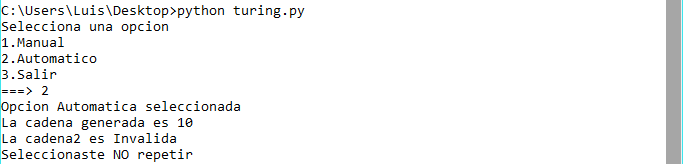
\includegraphics[width=\textwidth, height=8cm]{auto_turing}
\label{ }
\caption{Modo Automático}
\end{center}
\end{figure}

\begin{figure}[H]
\begin{center}
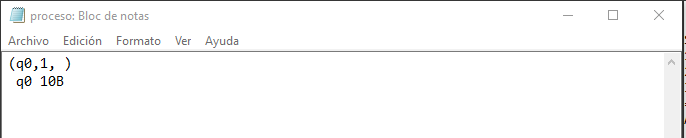
\includegraphics[width=\textwidth, height=8cm]{auto_turing_proceso}
\label{ }
\caption{Proceso por el cual pasa la máquina. }
\end{center}
\end{figure}

\begin{figure}[H]
\begin{center}
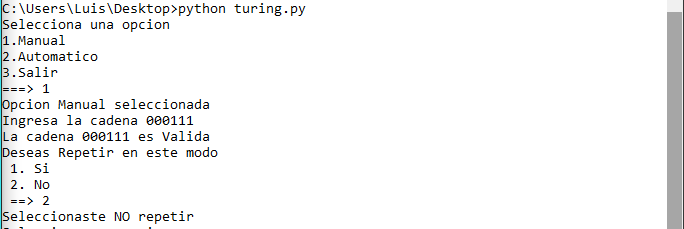
\includegraphics[width=\textwidth, height=8cm]{manual_turing}
\label{ }
\caption{Modo Manual}
\end{center}
\end{figure}

\begin{figure}[H]
\begin{center}
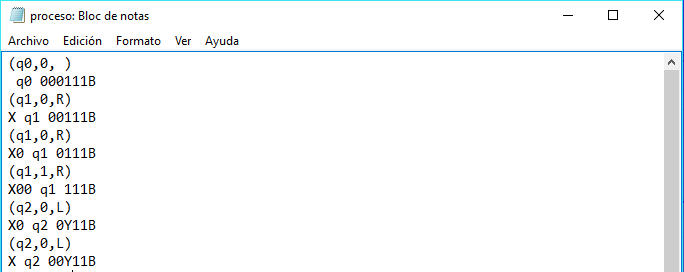
\includegraphics[width=\textwidth, height=8cm]{manual_turing_proceso}
\label{ }
\caption{Proceso por el cual pasa la máquina.}
\end{center}
\end{figure}

\begin{thebibliography}{9}
  \bibitem{Genaro} John E. Hopcroft, Rajeev Motwani, Jeffrey D. Ullman. (2007). Introducción a la teoría de autómatas, lenguajes y computación.. Madrid, España: PEARSON EDUCACIÓN.
\end{thebibliography}

%\bibliographystyle{acm}
%\bibliography{bibliografia}

\end{document}